\documentclass[twocolumn,11pt]{article}
\usepackage[margin=1in]{geometry}
\usepackage{graphicx}
\usepackage{multicol}
\usepackage{subcaption}
\usepackage{float}
\usepackage{amsmath}
\graphicspath{{./images/}}


\title{\vspace{-2cm}\Huge{Study of Algorithms to find the Nearest Neighbours under Periodic Boundary Conditions}}
\author{\Large{Pritipriya Dasbehera} \\ Roll no. 2111086 }


\begin{document}

\twocolumn[
  \begin{@twocolumnfalse}
    \maketitle
\begin{flushleft}
under the supervision of \emph{Dr. Nishikanta Khandai} and Project Report submitted to the School of Physical Sciences, \textbf{National Institute of Science Education and Research}, Bhubaneswar
\end{flushleft}
    \rule{\textwidth}{0.5pt}
    \begin{abstract}
Simulation of a large number of bodies in cosmology, hydrodynamics and aerodynamics involves considering a large number of interactions between them which almost always requires information of the nearest neighbours. The Periodic Boundary Conditions are used to simulate an infinite-size system by studying the dynamics of only a smaller part of it. This study is based on the implementation of two algorithms to find nearest neighbours: brute-force method and grid/sub-cell method, whose time-complexity is shown to be \(O(n^2)\) and \(O(n)\) respectively.
    \end{abstract}
    \rule{\textwidth}{0.5pt}
    \vspace{0.02in}
  \end{@twocolumnfalse}]

\section{Introduction}
In the case of hydrodynamics and aerodynamics, where short-range interaction is involved, only nearest neighbours can exert forces on a body. In the case of cosmology, where long-range gravitational interaction is involved, ideally, the interaction of each body with every other body should be considered. But that needs computation time of the order $O(n^{2})$, which is not feasible. Thus, the widely used approximation is to find the nearest neighbours of each body and consider the interaction between them. As for the bodies farther away, they can be clumped into groups and approximated as single bodies at the centre of mass of the groups [figure \ref{fig1}]. This reduces the calculation cost considerably depending on the algorithms used.
\begin{figure}
\centering
	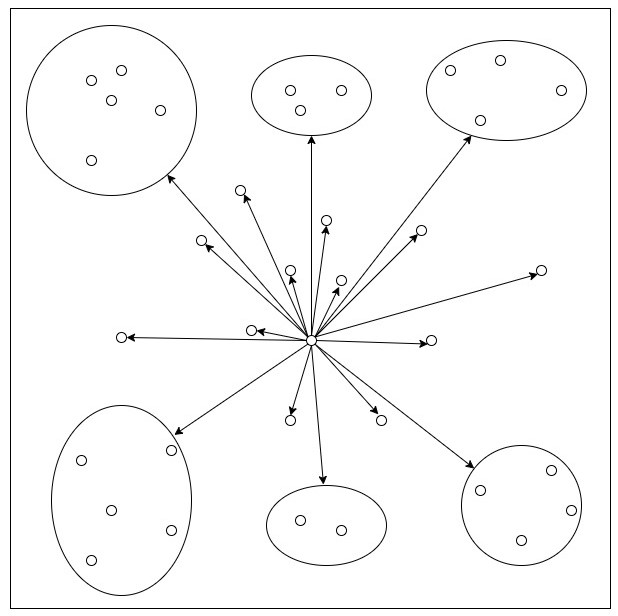
\includegraphics[width=0.9\linewidth]{nearest}
	\caption{\small{Approximating a long range interaction using nearest neighbours and grouping, in 2-D space}}
	\label{fig1}
\end{figure}

To simulate an infinitely large system, \textbf{Periodic Boundary Conditions} (PBC) are often used. Only a small unit of the system needs to be accounted for under PBC. The system is assumed to consist of infinitely many copies of these small units. When a body leaves the original unit, it reappears with the same velocity from the opposite direction. And each particle interacts only with the closest images of the remaining particles [Figure \ref{fig2}].
\begin{figure}
\centering
	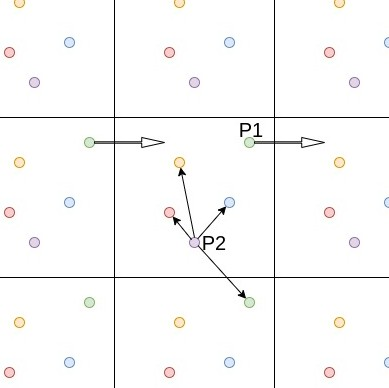
\includegraphics[width=0.85\linewidth]{PBC}
	\caption{\small{Periodic Boundary Conditions - When P1 moves out of the cell from the right, it enters from the left. Also the closest image of P1 for P2 is not in the original unit but in the sub-cell below it.}}
	\label{fig2}
\end{figure}

\section{Methodology}

\subsection{\textit{Distance calculation}}
If the two coordinates are $(x_{1},y_{1},z_{1})$ and $(x_{2},y_{2},z_{2})$ and length of cell is \(l\) then the effective distance is
\begin{equation}
ds = \sqrt[2]{dx^2 + dy^2 + dz^2}
\end{equation}
where
\begin{equation}
dx = \begin{cases}
|x_2 - x_1| &\text{if } |x_2-x_1| < l/2 \\
l - |x_2 - x_1| &\text{if } |x_2-x_1| \ge l/2
\end{cases}
\end{equation}
similarly for dy and dz.

But using if-else conditions in a program breaks the flow which makes parallelization difficult and may increase time, to avoid it the following equation is used\\
\begin{equation} 
dx = a_xl + (1 - 2a_{x})|x_2 - x_1|
\end{equation}
where\footnote{ $\lfloor \cdot \rfloor$ is the Greatest Integer Function}
\begin{equation}
a_x = \left\lfloor \frac{2|x_2-x_1|}{l} \right\rfloor = \begin{cases}
0 &\text{if } |x_2-x_1| < l/2 \\
1 &\text{if } |x_2-x_1| \ge l/2
\end{cases}
\end{equation}
similarly for dy and dz. From here on distance refers to effective distance unless stated otherwise.

\begin{figure}
\centering
	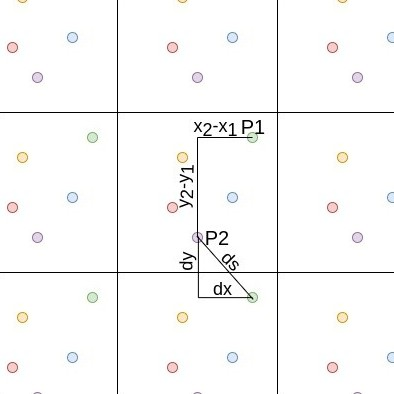
\includegraphics[width=0.85\linewidth]{dcalc}
	\caption{\small{Example of distance calculation in 2D where \( ds = \sqrt[2]{dx^2 + dy^2} \) .Here, $dx=|x_2-x_1| < l/2 $ but $dy=l - |y_2-y_1|$ as $|y_2-y_1|>l/2$}}
	\label{fig3}
\end{figure}

\subsection{\textit{Brute-force method}}
This method involves calculating the distances of each body to every other body and keeping track of the closest `k' bodies to it. This involves \( n^2 \) operations \footnote{This is independent of `k' the number of nearest neighbours required} where \(n\) is the total number of bodies. Thus this method should have time complexity $O(n^{2})$.

\subsection{\textit{Grid method}}
This method involves dividing the cell into a grid of smaller sub-cells and keeping track of the bodies in each sub-cell. If there are enough bodies in each sub-cell, then the nearest `k' bodies are present in the same sub-cell or sub-cells immediately surrounding it. If not, then they are in the $2^{nd}$ immediate surrounding sub-cells or the $3^{rd}$ immediate surrounding and so on [Figure \ref{fig4}].

For each body, about a constant number of sub-cells are checked for nearest neighbours. Thus, its time complexity should be $O(n)$.
\begin{figure}[h]
\centering
	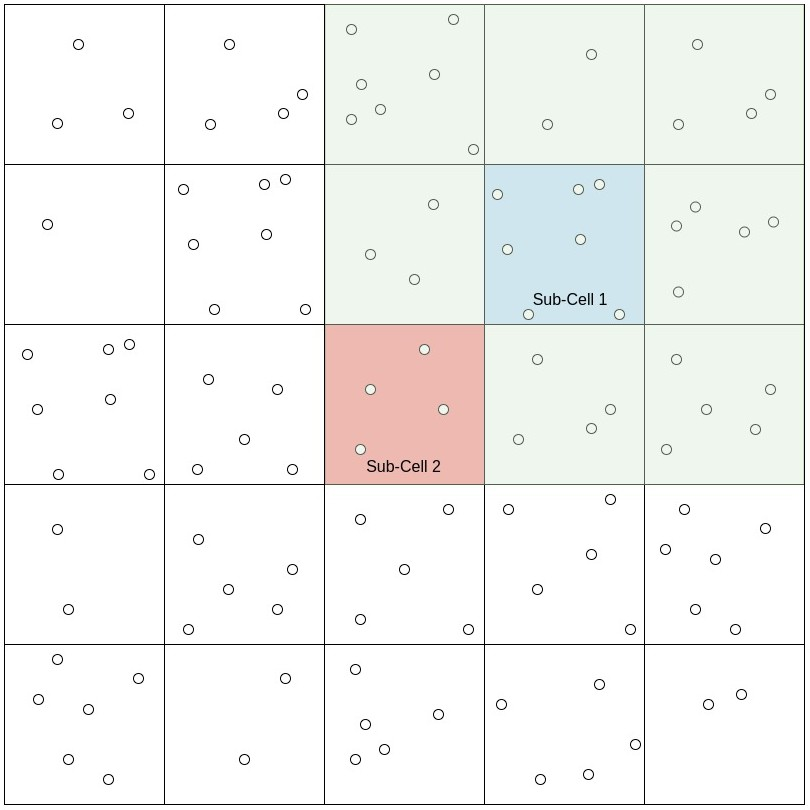
\includegraphics[width=0.9\linewidth]{grideg}
	\caption{\small{If a point in sub-cell 1 is considered with k=10, then the 3x3 subgrid(shaded), immediate surrounding, containing it will for sure have the nearest neighbours.\\ 
	For a point in sub-cell 2 and k=50, the 5x5 grid(whole grid), $2^{nd}$ immediate surrounding, will have the nearest neighbours.}}
	\label{fig4}
\end{figure}

\section{Results}
\subsection{\textit{Brute-force method}}
The plot of the program run-time(T) against the number of points (n) [Figure \ref{fig5}] is not linear.
\begin{figure}
\centering
	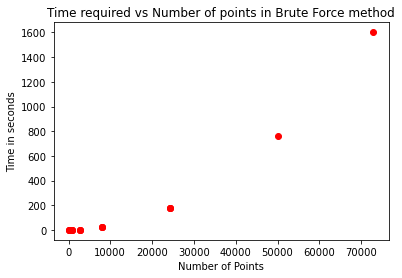
\includegraphics[width=0.9\linewidth]{brute}
	\caption{\small{Run-time against number of points for Brute-force method}}
	\label{fig5}
\end{figure}
To find the order of time complexity log plot is used. The log graph [figure \ref{fig7}] is straight line thus the dependence is of polynomial form (\(n^b\)) and not exponential (\(e^n\)). 

If the general form is considered to be 
\begin{equation} T = an^b \end{equation} then 
\begin{equation} log(T) = log(a) + blog(n) \end{equation}
which is a straight line for log(T) vs log(n) plot and has slope \(b\), which is the required order.

\begin{figure}[h]
\centering
	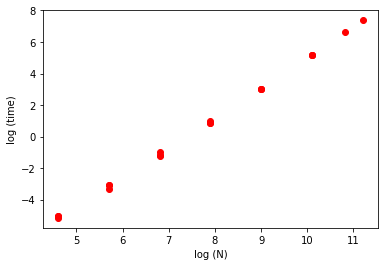
\includegraphics[width=0.9\linewidth]{brutelog}
	\caption{\small{log of run-time vs log of number of points for Brute-force method}}
	\label{fig6}
\end{figure}
The slope of best fit line is calculated (by iterative linear regression) to be 1.86, nearly equal to 2. \emph{This confirms time complexity of Brute-force method to be $O(n^{2})$}.
\begin{figure}[H]
\centering
	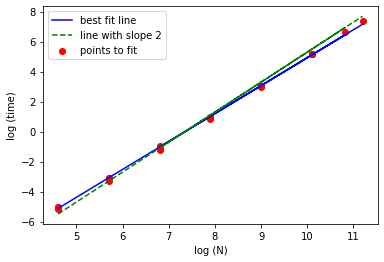
\includegraphics[width=0.9\linewidth]{brutefit}
	\caption{\small{Best fit line for log(T) vs log(n) graph}}
	\label{fig7}
\end{figure}

\newpage
\onecolumn
\begin{figure*}[h]
\centering
	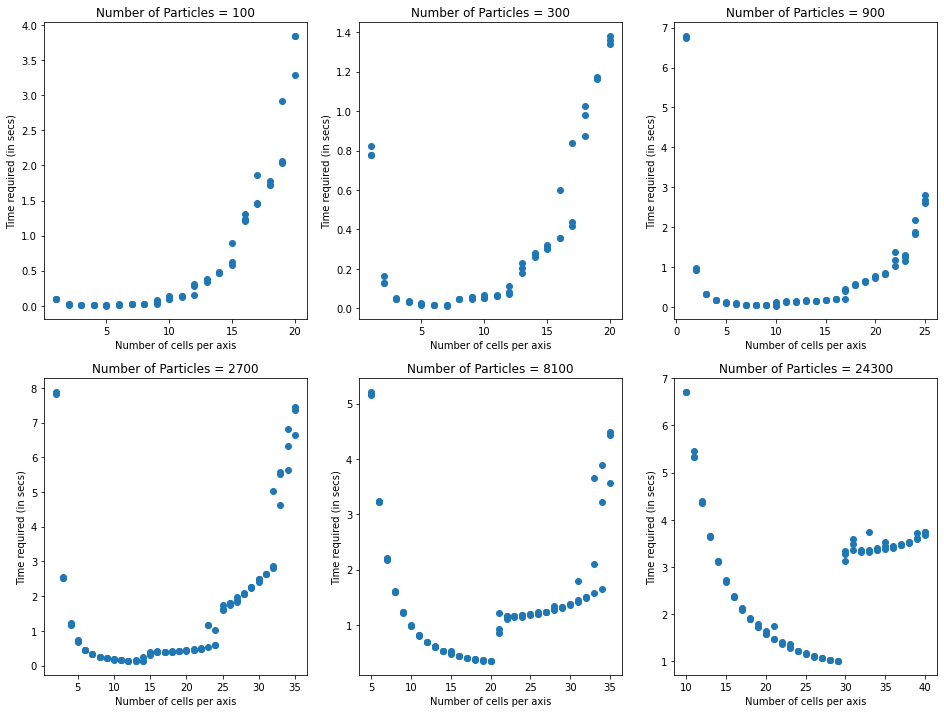
\includegraphics[width=\linewidth]{gridperaxis}
	\caption{\small{Run-time vs number of sub-cells per axis for different number of points}}
	\label{fig8}
\end{figure*}
\begin{multicols}{2}
\subsection{\textit{Ideal number of sub-cells per axis for Grid method}}
The grid method requires dividing the cell into sub-cells [Figure \ref{fig9}]. If the number of sub-cells is too many, then each sub-cell contains less number of points/bodies. A larger sub-grid will have to be searched to find the nearest neighbours. If the number of cells is too few, then each sub-cell has many points, and a larger number of calculations need to be done. So there exists an ideal number of sub-cells which requires the least run-time. This is evident from the figure \ref{fig8}.\\

By taking the ideal number of sub-cells (the number of sub-cells per axis with the least run-time) from figure \ref{fig8}, a plot can be made to find the relation between the number of sub-cells per axis and the total number of points/bodies.


\begin{center}
  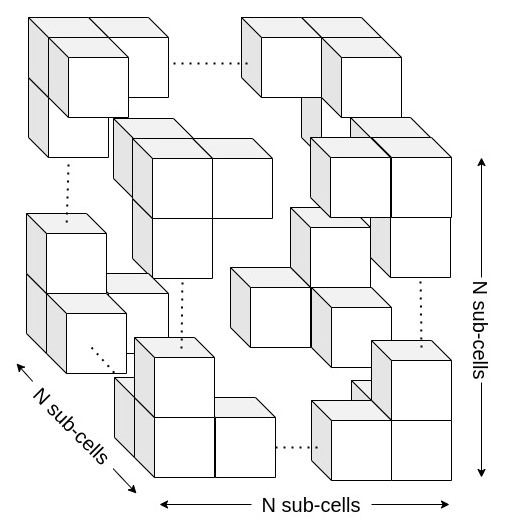
\includegraphics[width=0.9\linewidth]{gridn}
  \captionof{figure}{\small{\(N\) sub-cells per axis means total \(N^3\) sub-cells}}
  \label{fig9}
\end{center}

\end{multicols}
\twocolumn

\begin{figure}
\centering
	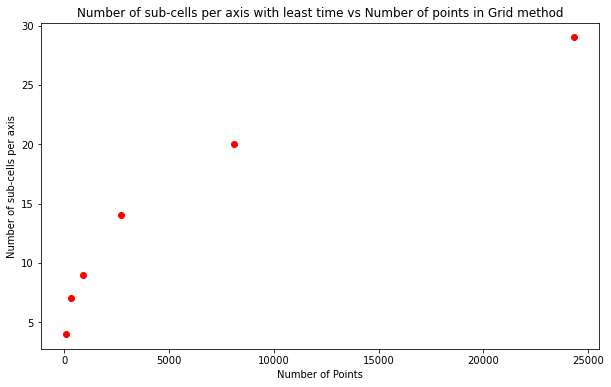
\includegraphics[width=\linewidth]{subcell}
	\caption{\small{Number of sub-cells per axis vs Total number of points/bodies}}
	\label{fig10}
\end{figure}
The plot [figure \ref{fig10}] of sub-cells per axis vs the number of points is not linear, but the log plot [figure \ref{fig11}] is linear. Thus the relation is of polynomial form.
\begin{figure}[h]
\centering
	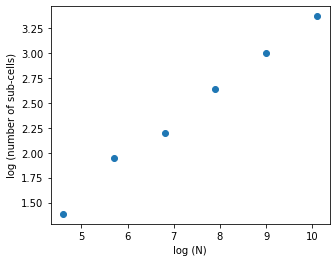
\includegraphics[width=\linewidth]{subcelllog}
	\caption{\small{log of number of sub-cells per axis vs log of number of points}}
	\label{fig11}
\end{figure}

\begin{figure}[h]
\centering
	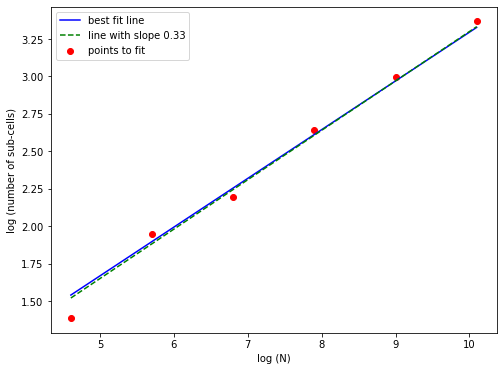
\includegraphics[width=\linewidth]{subcellfit}
	\caption{\small{best fit line for the log(sub-cells) vs log(n) plot has slope nearly 0.33 and intercept 0}}
	\label{fig12}
\end{figure}

Considering the dependence to be
\begin{equation} N = an^b \end{equation}
where \(N=\) Number of sub-cells per axis and \\ \(n=\) Total number of points/bodies.
\begin{equation} log(N) = log(a) + blog(n) \end{equation}

From the slope and intercept of best fit line [Figure \ref{fig12}], \(b=0.33\) and \(a=1\) i.e.
\begin{equation} N = n^{0.33} \end{equation}

\subsection{\textit{Grid method}}
Now that the optimum number of sub-cells is known, the run-time of the grid method for different numbers of points/bodies can be plotted[Figure \ref{fig13}], which turns out to be linear. \emph{This confirms the time complexity of the grid method to be $O(n)$}.
\begin{figure}[h]
\centering
	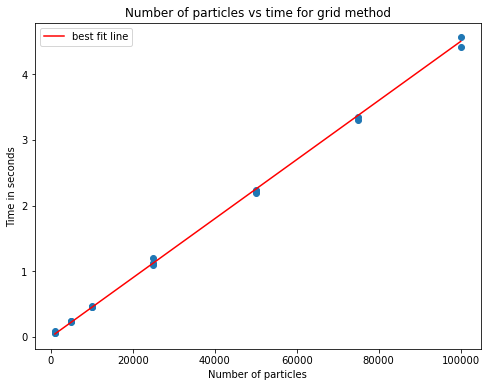
\includegraphics[width=\linewidth]{gridfit}
	\caption{\small{best fit line for run-time vs number of points}}
	\label{fig13}
\end{figure}

\newpage
\onecolumn
\begin{figure*}[h]
\centering
	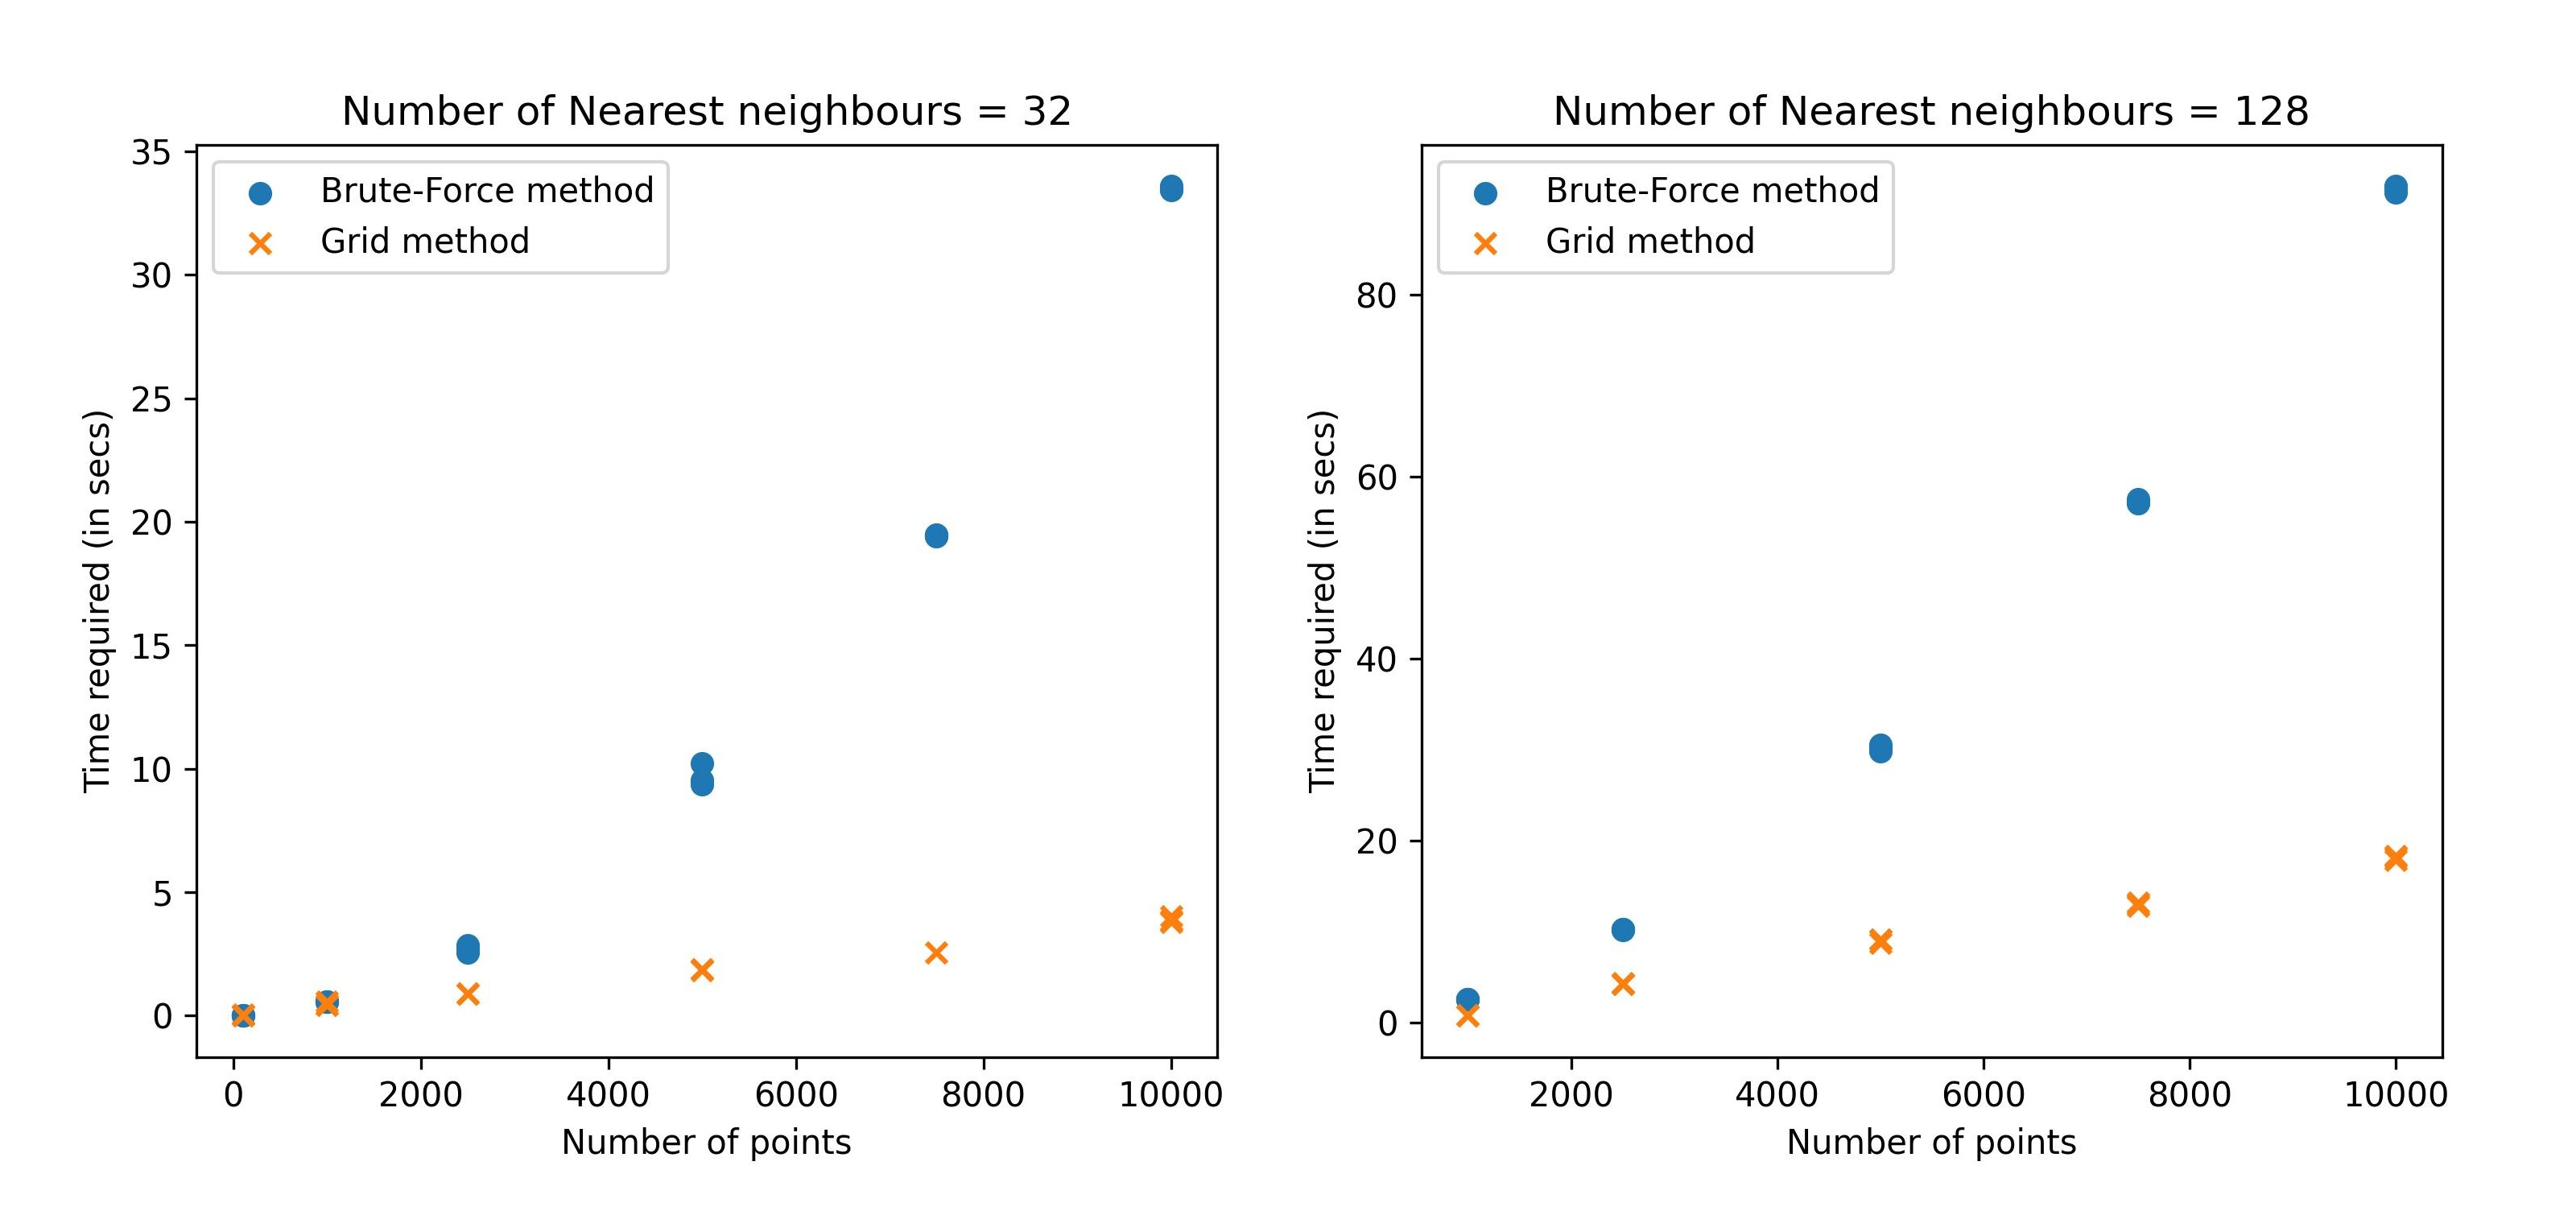
\includegraphics[width=1\linewidth]{fig}
	\caption{\small{Comparing the two methods for different number of points/bodies}}
	\label{fig14}
\end{figure*}
\begin{multicols}{2}
\section{Conclusion}
Comparing the two methods[Figure \ref{fig14}] we can observe that both methods perform equally well when the number of points/bodies is less. As the number of points/bodies increases, the difference in time becomes more significant and the superiority of the grid method becomes evident.
\end{multicols}
\rule{\textwidth}{0.5pt}
\end{document}

\section*{Appendix I - Brute Force Source Code (Rust)}
\begin{verbatim}
use std::io::prelude::*;
use std::fs::File;
use std::time::{self, Duration};
use rand::Rng;

const NUM_OF_PARTICLES: usize = 100;
const NEAREST_NEIGHBOURS_REQ: usize = 10;
const MAX_DIST: f64 = 0.8660254037844387;

fn main() {
    let mut now = time::Instant::now();
    let zeropt =  Point{x:0.0,y:0.0,z:0.0};
    let mut points  = vec![zeropt;NUM_OF_PARTICLES];
    point_generator(&mut points);
    let t_point_create = now.elapsed();
    println!("The time taken to create {} particles is {}
microseconds.",NUM_OF_PARTICLES,t_point_create.as_micros());

    now = time::Instant::now();
    write_points(&points);
    let t_point_write = now.elapsed();
    println!("The time taken to write {} particles is {}
microseconds.",NUM_OF_PARTICLES,t_point_write.as_micros());

    now = time::Instant::now();
    let mut nearlist = vec![Node{id:0,dist:MAX_DIST};
    (NEAREST_NEIGHBOURS_REQ+1)*NUM_OF_PARTICLES];
    let t_init = now.elapsed();
    println!("The time taken to initialise {} particle nearlist is {}
microseconds.",NUM_OF_PARTICLES,t_init.as_micros());

    now = time::Instant::now();
    brute_cal_nearest(&points, &mut nearlist);
    let t_brute = now.elapsed();
    println!("The time taken to brute calc {} particle nearlist is {} 
microseconds.",NUM_OF_PARTICLES,t_brute.as_micros());

    now = time::Instant::now();
    write_nearlist(&nearlist);
    let elapsed_time = now.elapsed();
    println!("The time taken to write {} particle nearlist is {} 
microseconds.",NUM_OF_PARTICLES,elapsed_time.as_micros());

    write_time(t_point_create, t_point_write, t_init, t_brute);
}

// #[derive(Debug)]
#[derive(Clone, Copy)]
struct Point{x: f64,y:f64,z:f64}

#[derive(Debug)]
#[derive(Clone, Copy)]
struct Node{id: u32, dist: f64}

fn dist(p1:&Point ,p2:&Point)->f64{
    let mut dx = (p1.x -p2.x).abs();
    let ax: f64 = (dx / 0.5 ).floor();
    dx = ax + (1.0 - 2.0 * ax) * dx;

    let mut dy = (p1.y -p2.y).abs();
    let ay: f64 = {dy / 0.5 }.floor();
    dy = ay + (1.0 - 2.0 * ay) * dy;


    let mut dz = (p1.z -p2.z).abs();
    let az: f64 = {dz / 0.5 }.floor();
    dz = az + (1.0 - 2.0 * az) * dz;


fn point_generator(points: &mut Vec<Point>){
    for (_i,element) in points.iter_mut().enumerate(){
        element.x = rand::thread_rng().gen::<f64>();
        element.y = rand::thread_rng().gen::<f64>();
        element.z = rand::thread_rng().gen::<f64>();
    }

}


fn write_points(points: &Vec<Point>){
    let mut file = File::create("points.csv").expect("Something went 
wrong in file creation");
    file.write_all(b"id,x,y,z\n").expect("unable to write");
    for (i,element) in points.iter().enumerate(){
        let mut data = String::new();
        data.push_str(&i.to_string());
        data.push(',');
        data.push_str(&element.x.to_string());
        data.push(',');
        data.push_str(&element.y.to_string());
        data.push(',');
        data.push_str(&element.z.to_string());
        data.push('\n');
        file.write_all(data.as_bytes()).expect("unable to write");
    }
}

fn write_nearlist(nearlist:&Vec<Node>){
    let mut file = File::create("nearlist.csv").expect("Something went wrong
 in file creation");
    for i in 0..NUM_OF_PARTICLES //*(NEAREST_NEIGHBOURS_REQ+1)
    {
        let mut data = String::new();
        for (j,element) in nearlist[i*(NEAREST_NEIGHBOURS_REQ+1)..i*
(NEAREST_NEIGHBOURS_REQ+1)+NEAREST_NEIGHBOURS_REQ].iter().enumerate(){
            if j==0{data.push_str(&i.to_string());continue};
            if j==NEAREST_NEIGHBOURS_REQ+1{break;};
            data.push(',');
            data.push_str(&element.id.to_string());
        }
        data.push('\n');
        file.write_all(data.as_bytes()).expect("unable to write");
    }
}

fn write_time(t_point_create:Duration,t_point_write:Duration,t_init:Duration,
t_brute:Duration){
    let mut file = File::options().append(true).open("time.csv").expect("Something went 
wrong in file creation");
    let mut data = String::new();
    data.push_str(&NUM_OF_PARTICLES.to_string());
    data.push(',');
    data.push_str(&t_point_create.as_micros().to_string());
    data.push(',');
    data.push_str(&t_point_write.as_micros().to_string());
    data.push(',');
    data.push_str(&t_init.as_micros().to_string());
    data.push(',');
    data.push_str(&t_brute.as_micros().to_string());
    data.push('\n');
    file.write_all(data.as_bytes()).expect("unable to write");

}

fn brute_cal_nearest(points: &Vec<Point>, nearlist:&mut Vec<Node>){
    for i in 0..NUM_OF_PARTICLES
    {
        for j in 0..NUM_OF_PARTICLES
        {
            if i == j
            {
                continue;
            }
            let d = dist(&points[i],&points[j]);
            // print!("The distance between point {i} and point {j} is {d}\n");
            if d<nearlist[i*(NEAREST_NEIGHBOURS_REQ+1)].dist{
                // print!("Inserting node for {i}\t");
                let mut k = 1;
                while k<NEAREST_NEIGHBOURS_REQ && nearlist[i*
(NEAREST_NEIGHBOURS_REQ+1)+k].dist < d{
                    k+=1;
                }
                nearlist[i*(NEAREST_NEIGHBOURS_REQ+1)+k..=i*
(NEAREST_NEIGHBOURS_REQ+1)+NEAREST_NEIGHBOURS_REQ].rotate_right(1);
                nearlist[i*(NEAREST_NEIGHBOURS_REQ+1)+k] = Node{id:j as u32,dist:d};
                nearlist[i*(NEAREST_NEIGHBOURS_REQ+1)].dist = 
nearlist[i*(NEAREST_NEIGHBOURS_REQ+1)+NEAREST_NEIGHBOURS_REQ].dist;
            }
        }
        // let mut data = String::new();
        // for (j,element) in nearlist[i].iter().enumerate(){
        //     if j==0{data.push_str(&i.to_string());continue};
        //     if j==NEAREST_NEIGHBOURS_REQ+1{break;};
        //     data.push_str(",");
        //     data.push_str(&element.id.to_string());
        // }
        // data.push_str("\n");
        // file.write_all(data.as_bytes()).expect("unable to write");
    }
}
\end{verbatim}
\newpage
\section*{Appendix II - Grid Method Source Code (Rust)}
\begin{verbatim}
use std::io::prelude::*;
use std::fs::File;
use std::time::{self, Duration};
use rand::Rng;
use ndarray::{Array3};

const NUM_OF_PARTICLES: usize = 1000000;
const NEAREST_NEIGHBOURS_REQ: usize = 10;
const MAX_DIST: f64 = 0.8660254037844387;
const GRID_SIZE: usize = 44;
const GRID_LEN: f64 = 1.0/44.0;

fn main() {
    let mut now = time::Instant::now();
    let _z = now;
    let zeropt =  Point{x:0.0,y:0.0,z:0.0};
    let mut points  = vec![zeropt;NUM_OF_PARTICLES];
    point_generator(&mut points);
microseconds.",NUM_OF_PARTICLES,t_point_create.as_micros());

    // now = time::Instant::now();
    write_points(&points);
    // let t_point_write = now.elapsed();
    // println!("The time taken to write {} particles is {} microseconds.",
NUM_OF_PARTICLES, t_point_write.as_micros());

    // now = time::Instant::now();
    let mut nearlist = vec![Node{id:0,dist:MAX_DIST};
(NEAREST_NEIGHBOURS_REQ+1)*NUM_OF_PARTICLES];
    // let t_init = now.elapsed();
    // println!("The time taken to initialise {} particle nearlist is {} 
microseconds.",NUM_OF_PARTICLES,t_init.as_micros());
    // print_nearlist(&nearlist);

    now = time::Instant::now();
    let mut grid = Array3::from_elem((GRID_SIZE,GRID_SIZE,GRID_SIZE), vec![0_usize]);
    create_grid(&points, &mut grid);
    let t_grid = now.elapsed();
    // println!("The time taken to make grid of {} particles is {} 
microseconds.",NUM_OF_PARTICLES,t_grid.as_micros());

    write_grid(&grid);

    now = time::Instant::now();
    grid_calc_nearest(&points, &grid, &mut nearlist);
    let t_gridcalc = now.elapsed();
    // println!("The time taken to grid calc {} particle nearlist is {} 
microseconds.",NUM_OF_PARTICLES,t_gridcalc.as_micros());

    // now = time::Instant::now();
    // brute_cal_nearest(&points, &mut nearlist);
    // let t_brute = now.elapsed();
    // println!("The time taken to brute calc {} particle nearlist is {} 
microseconds.",NUM_OF_PARTICLES,t_brute.as_micros());

    // now = time::Instant::now();
    write_nearlist(&nearlist);
    // let elapsed_time = now.elapsed();
    // println!("The time taken to write {} particle nearlist is {} 
microseconds.",NUM_OF_PARTICLES,elapsed_time.as_micros());

    // write_time(t_point_create, t_point_write, t_init, t_grid+t_gridcalc);
    write_gridtime(t_grid,t_gridcalc);
}

// #[derive(Debug)]
#[derive(Clone, Copy)]
struct Point{x: f64,y:f64,z:f64}

#[derive(Debug)]
#[derive(Clone, Copy)]
struct Node{id: u32, dist: f64}

fn dist(p1:&Point ,p2:&Point)->f64{
    let mut dx = (p1.x -p2.x).abs();
    let ax: f64 = (dx / 0.5 ).floor();
    dx = ax + (1.0 - 2.0 * ax) * dx;

    let mut dy = (p1.y -p2.y).abs();
    let ay: f64 = {dy / 0.5 }.floor();
    dy = ay + (1.0 - 2.0 * ay) * dy;


    let mut dz = (p1.z -p2.z).abs();
    let az: f64 = {dz / 0.5 }.floor();
    dz = az + (1.0 - 2.0 * az) * dz;

    dx.powf(2.0) + dy.powf(2.0) + dz.powf(2.0)
}

fn point_generator(points: &mut Vec<Point>){

    // let mut file = File::create("points.csv").expect("Something 
went wrong in file creation");
    // let mut file = File::options().append(true).open("points.csv")
.expect("Something went wrong in file creation");
    for (_i,element) in points.iter_mut().enumerate(){
        element.x = rand::thread_rng().gen::<f64>();
        element.y = rand::thread_rng().gen::<f64>();
        element.z = rand::thread_rng().gen::<f64>();
    }

}

fn write_points(points: &Vec<Point>){
    let mut file = File::create("points.csv").expect("Something went 
wrong in file creation");
    file.write_all(b"id,x,y,z\n").expect("unable to write");
    for (i,element) in points.iter().enumerate(){
        let mut data = String::new();
        data.push_str(&i.to_string());
        data.push(',');
        data.push_str(&element.x.to_string());
        data.push(',');
        data.push_str(&element.y.to_string());
        data.push(',');
        data.push_str(&element.z.to_string());
        data.push('\n');
        file.write_all(data.as_bytes()).expect("unable to write");
        
        // let row = concat!(i.to_string,b",",element.x.to_be_bytes);
        // let str = i.to_be_bytes()+",".as_bytes()+element.x.to_be_bytes();
    }
}

fn write_nearlist(nearlist:&Vec<Node>){
    let mut file = File::create("nearlist.csv").expect("Something 
went wrong in file creation");
    // let mut file = File::options().append(true).open("nearlist.csv")
.expect("Something went wrong in file creation");
    // for (i, _element) in nearlist.iter().enumerate().take(NUM_OF_PARTICLES)
    for i in 0..NUM_OF_PARTICLES //*(NEAREST_NEIGHBOURS_REQ+1)
    {
        let mut data = String::new();
        for (j,element) in nearlist[i*(NEAREST_NEIGHBOURS_REQ+1)..i*
(NEAREST_NEIGHBOURS_REQ+1)+NEAREST_NEIGHBOURS_REQ].iter().enumerate(){
            if j==0{data.push_str(&i.to_string());continue};
            if j==NEAREST_NEIGHBOURS_REQ+1{break;};
            data.push(',');
            data.push_str(&element.id.to_string());
        }
        data.push('\n');
        file.write_all(data.as_bytes()).expect("unable to write");
    }
}

// fn write_time(t_point_create:Duration,t_point_write:Duration,
t_init:Duration,t_brute:Duration){
//     let mut file = File::options().append(true).open("time.csv")
.expect("Something went wrong in file creation");
//     let mut data = String::new();
//     data.push_str(&NUM_OF_PARTICLES.to_string());
//     data.push(',');
//     data.push_str(&t_point_create.as_micros().to_string());
//     data.push(',');
//     data.push_str(&t_point_write.as_micros().to_string());
//     data.push(',');
//     data.push_str(&t_init.as_micros().to_string());
//     data.push(',');
//     data.push_str(&t_brute.as_micros().to_string());
//     data.push('\n');
//     file.write_all(data.as_bytes()).expect("unable to write");
// }

fn write_gridtime(t_grid:Duration,t_gridcalc:Duration){
    let mut file = File::options().append(true).open("gridtime2.csv")
.expect("Something went wrong in file creation");
    let mut data = String::new();
    data.push_str(&NUM_OF_PARTICLES.to_string());
    data.push(',');
    data.push_str(&GRID_SIZE.to_string());
    data.push(',');
    data.push_str(&t_grid.as_micros().to_string());
    data.push(',');
    data.push_str(&t_gridcalc.as_micros().to_string());
    data.push('\n');
    file.write_all(data.as_bytes()).expect("unable to write");
}

fn create_grid(points: &[Point], grid:&mut Array3<Vec<usize>>){
    for (i,point) in points.iter().enumerate(){
        let x = (point.x/GRID_LEN) as usize;
        let y = (point.y/GRID_LEN) as usize;
        let z = (point.z/GRID_LEN) as usize;
        
        grid[[x,y,z]][0] += 1;
        let index = grid[[x,y,z]][0];
        grid[[x,y,z]].insert(index, i);
    }
}

fn write_grid(grid:&Array3<Vec<usize>>){
    let mut file = File::create("grid.csv").expect("Something 
went wrong in file creation");
    for cell in grid.iter(){
        let mut data = String::new();
        for id in cell.iter(){
            data.push_str(&id.to_string());
            data.push(',')
        }
        data.push('\n');
        file.write_all(data.as_bytes()).expect("Couldnt write the points");
    }
}

// fn write_grid(grid:&Array3<Vec<usize>>){
//     let mut file = File::create("nearlist.csv").expect("Something went
wrong in file creation");
//     {0..GRID_SIZE}.for_each(|i|
//         {0..GRID_SIZE}.for_each(|j|
//             {0..GRID_SIZE}.for_each(|k|{
//                 file.write_all();
//             }
//             )))
// }

// fn brute_cal_nearest(points: &Vec<Point>, nearlist:&mut Vec<Node>){
//     for i in 0..NUM_OF_PARTICLES
//     {
//         for j in 0..NUM_OF_PARTICLES
//         {
//             if i == j
//             {
//                 continue;
//             }
//             let d = dist(&points[i],&points[j]);
//             // print!("The distance between point {i} and point {j} is {d}\n");
//             if d<nearlist[i*(NEAREST_NEIGHBOURS_REQ+1)].dist{
//                 // print!("Inserting node for {i}\t");
//                 let mut k = 1;
//                 while k<NEAREST_NEIGHBOURS_REQ && nearlist[i*
(NEAREST_NEIGHBOURS_REQ+1)+k].dist < d{
//                     k+=1;
//                 }
//                 nearlist[i*(NEAREST_NEIGHBOURS_REQ+1)+k..=i*
(NEAREST_NEIGHBOURS_REQ+1)+NEAREST_NEIGHBOURS_REQ].rotate_right(1);
//                 nearlist[i*(NEAREST_NEIGHBOURS_REQ+1)+k] = Node{id:j as u32,dist:d};
//                 nearlist[i*(NEAREST_NEIGHBOURS_REQ+1)].dist =
nearlist[i*(NEAREST_NEIGHBOURS_REQ+1)+NEAREST_NEIGHBOURS_REQ].dist;
//                 // print_nearlist(nearlist);
//                 // println!("\n");
//             }
//         }
//         // let mut data = String::new();
//         // for (j,element) in nearlist[i].iter().enumerate(){
//         //     if j==0{data.push_str(&i.to_string());continue};
//         //     if j==NEAREST_NEIGHBOURS_REQ+1{break;};
//         //     data.push_str(",");
//         //     data.push_str(&element.id.to_string());
//         // }
//         // data.push_str("\n");
//         // file.write_all(data.as_bytes()).expect("unable to write");
//     }
// }

fn grid_calc_nearest(points: &Vec<Point>,grid:&Array3<Vec<usize>>, 
nearlist:&mut Vec<Node>, ){
    let mut buffer: i64 = 1;
    (0..GRID_SIZE).for_each(|i|{
        (0..GRID_SIZE).for_each(|j|{
            (0..GRID_SIZE).for_each(|k|{
                let mut size:usize = grid[[i,j,k]].len();
                loop{
                    if size>=NEAREST_NEIGHBOURS_REQ{break;}
                    size = 0;
                    (i as i64-buffer..=i as i64+buffer).for_each(|mut ti|
                        (j as i64-buffer..=j as i64+buffer).for_each(|mut tj|
                            (k as i64-buffer..=k as i64+buffer).for_each(|mut tk|{
                                if ti < 0 {ti = GRID_SIZE as i64+ti} 
                                else if ti >= GRID_SIZE as i64 {ti = ti - GRID_SIZE as i64};
                                if tj < 0 {tj = GRID_SIZE as i64+tj} 
                                else if tj >= GRID_SIZE as i64 {tj = tj - GRID_SIZE as i64};
                                if tk < 0 {tk = GRID_SIZE as i64+tk} 
                                else if tk >= GRID_SIZE as i64 {tk = tk - GRID_SIZE as i64};
                                let ti = ti as usize;
                                let tj = tj as usize;
                                let tk = tk as usize;
                                // println!("The size is {size}");
                                size += grid[[ti,tj,tk]][1..].len();
                                // println!("The size is {size}");
                            })
                        )
                    );
                    // println!("The size is finally {size}\n\n");
                    if size>=NEAREST_NEIGHBOURS_REQ{break;}
                    // println!("Inside loop");
                    buffer+=1;
                };
                // println!("Grid {i},{j},{k} has buffer {buffer}");
                grid[[i,j,k]][1..].iter().for_each(|point1_id|{
                    let point1_id=point1_id.clone();
                    // println!("Comparing from point{point1_id}");
                    (i as i64-buffer..=i as i64+buffer).for_each(|mut ti|
                        (j as i64-buffer..=j as i64+buffer).for_each(|mut tj|
                            (k as i64-buffer..=k as i64+buffer).for_each(|mut tk|{
                                if ti < 0 {ti = GRID_SIZE as i64+ti} 
                                else if ti >= GRID_SIZE as i64 {ti = ti - GRID_SIZE as i64};
                                if tj < 0 {tj = GRID_SIZE as i64+tj} 
                                else if tj >= GRID_SIZE as i64 {tj = tj - GRID_SIZE as i64};
                                if tk < 0 {tk = GRID_SIZE as i64+tk} 
                                else if tk >= GRID_SIZE as i64 {tk = tk - GRID_SIZE as i64};
                                let ti = ti as usize;
                                let tj = tj as usize;
                                let tk = tk as usize;
                                for point2_id in grid[[ti,tj,tk]][1..].iter(){
                                    let point2_id=point2_id.clone();
                                    if point1_id==point2_id{continue;} 
                                    let d = dist(&points[point1_id],&points[point2_id]);
                                    if d<nearlist[point1_id*(NEAREST_NEIGHBOURS_REQ+1)].dist{
                                        // print!("Inserting node for {i}\t");
                                        let mut k = 1;
                                        while k<NEAREST_NEIGHBOURS_REQ &&
 nearlist[point1_id*(NEAREST_NEIGHBOURS_REQ+1)+k].dist < d {k+=1;}
                                        nearlist[point1_id*(NEAREST_NEIGHBOURS_REQ+1)
+k..=point1_id*(NEAREST_NEIGHBOURS_REQ+1)+NEAREST_NEIGHBOURS_REQ].rotate_right(1);
                                        nearlist[point1_id*(NEAREST_NEIGHBOURS_REQ+1)+k] =
 Node{id:point2_id as u32,dist:d};
                                        nearlist[point1_id*(NEAREST_NEIGHBOURS_REQ+1)].dist = 
nearlist[point1_id*(NEAREST_NEIGHBOURS_REQ+1)+NEAREST_NEIGHBOURS_REQ].dist;
                                    }
                                }
                            })
                        )
                    );
                });
            })
        })
    });
}
\end{verbatim}